\documentclass[11pt,twoside,titlepage]{article}
\usepackage[tc]{titlepic}
\usepackage{times}
\usepackage{float}
\usepackage{amssymb}
\usepackage{amsmath}
\usepackage{amsthm}
\usepackage{needspace}
\usepackage{url}
\usepackage{hyperref}
%\usepackage{mathptm}
\usepackage{fancyhdr}
\usepackage{wrapfig}
\ifx\pdfoutput\undefined
% we are running LaTeX, not pdflatex
\usepackage{epsfig,color}
\else
% we are running pdflatex, so convert .eps files to .pdf
\usepackage[pdftex]{epsfig,color}
\usepackage{epstopdf}
\usepackage{pdfsync}
\fi
\usepackage{ifthen,version}
\usepackage{listings}
\usepackage{setspace}





%\usepackage{temporal}
%\usepackage{algorithmic}
\newboolean{print-solutions}

% Start of configuration section
% Comment out the following line to exclude the printing of solutions.
%\setboolean{print-solutions}{true}
\newcommand{\labnumber}{1}
\newcommand{\labname}{Digital Logic Gates}
\newcommand{\coursenumber}{Zybo Z7-10 and Vivado How-To Document}
\newcommand{\coursename}{Introduction to Digital Design}
% End of configuration section

% Conditional definitions
\newcommand{\dateorsol}{\LARGE \ifthenelse{\boolean{print-solutions}}%
  {Solutions}{Due \duedate}}
\newcommand{\headertxt}{\sl \ifthenelse{\boolean{print-solutions}}%
  {Solutions to}{} Laboratory Exercise \#\labnumber}
\newcommand{\points}[1]{\ifthenelse{\boolean{print-solutions}}%
  {}{[#1 points.]}}
\ifthenelse{\boolean{print-solutions}}{\includeversion{prnt-solns}}%
{\excludeversion{prnt-solns}}

\textwidth=7.25in
\evensidemargin=-0.35in
\oddsidemargin=-0.35in

\newcommand{\ite}{\operatorname{ite}}
\newcommand{\itec}{\operatorname{ite\_constant}}

{\theoremstyle{definition} \newtheorem{definition}{Definition}}
\newtheorem{theorem}{Theorem}
\newtheorem{lemma}{Lemma}
\newtheorem{corollary}{Corollary}
\newtheorem{proposition}{Proposition}
{\theoremstyle{remark}
  \newtheorem{example}{Example}
  \newtheorem{problem}{Problem}
  \newtheorem{note}{Note}}
% Fortunately, proofs can be nested.
\newenvironment{solution}{\begin{proof}[Solution]}{\end{proof}}

\newcommand{\ta}{Created By: Kyler Scott and Prof. Sunil P. Khatri\\July 2020}
\title{ \huge Department of Electrical and Computer Engineering\\ \huge Texas A\&M University \\}
\author{ \huge Zybo Z7-10 and Vivado:\\ \\ \huge How-To Document \\ \\ \\ \\ \ta}

\titlepic{
\includegraphics[width=0.5\textwidth]{logo}}

\date{}
\pagestyle{fancy}
\lhead[\rm\thepage]{}
\rhead[]{\rm\thepage}
\lfoot[]{\coursenumber}
%\cfoot{\instructor}
\rfoot[\coursenumber]{}

\begin{document}
\bibliographystyle{alpha}
\maketitle


\section{Introduction}

The Zybo Z7-10 FPGA board is an embedded software and digital circuit development board built around the Xilinx Zynq-7000 family. The Zynq family is based on the Xilinx All Programmable System-on-Chip (AP SoC) architecture, which integrates a dual-core ARM Cortex-A9 processor with Xilinx 7-series Field Programmable Gate Array (FPGA) logic. \\

\noindent
During the ECEN 248 and ECEN 449/749 labs, we will use the Zybo Z7-10 to accomplish various tasks, including simulating and sythesizing Verilog modules and running software which interfaces with these modules. To use the Zybo Z7-10 board, you will need to install "Vivado 2018.3", which is the software provided by Xilinx to communicate with the Zybo Z7-10. Consult the "Vivado 2018.3 Installation How-To Document" for help with this.\\

\noindent
This guide will cover some functionality of the Zybo Z7-10, which we will access and program using Vivado 2018.3. It is intended to impart a basic understanding of the tools needed for the ECEN 248 and ECEN 449/749 labs. The topics covered in this guide are as follows.

\begin{itemize}
\item Simulating a Verilog module with a test bench
\item Connecting buttons, switches, and other ports to a Verilog module and synthesizing the module onto the FPGA
\item Creation of a block design and using the Software Design Kit (SDK)
\item Creation of custom IP
\end{itemize}

\noindent
ECEN 248 should do the exercises in sections 2 and 3; ECEN 449/749 students should do the exercises in sections 2, 3, 4, and 5.\\

\section{Simple Verilog Source Code: Simulate and Verify with Test Bench} 

\noindent
In this section, we will create a simple Vivado project which implements a binary counter in Verilog and tests the functionality of the counter using a test bench. 

\begin{enumerate}
	\item Launch Vivado and create a new design project.
	\begin{enumerate}
		\item To begin, open Vivado 2018.3, and once it loads, select \textbf{File} $\rightarrow$ \textbf{New Project} \\
		The New Project Wizard will open. Click `Next' and a window as in Figure~\ref{newproj} will open.  \\
		
		
		\begin{figure}[!h]
			\centering
			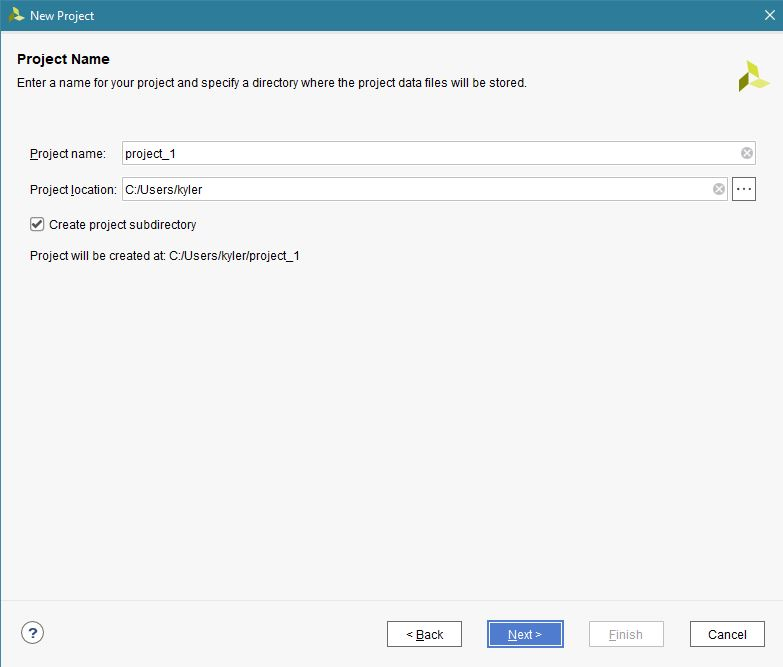
\includegraphics[width=.7\textwidth]{newproj}
			\caption{New Project Window}
			\label{newproj}
		\end{figure}
	
		\item Type a Project Name (ex. zybo\_test) and a Project Location. Click `Next' and select `RTL Project'. Click `Next'  and the `Add Sources' window will appear. Select Target language as `Verilog' and simulator language as `Verilog'. Click `Next' until you reach  the `Default Part' window. As shown in Figure~\ref{boards}, select 'Family' as 'Zynq-7000', 'Package' as 'clg400' and 'Speed' as '-1'. Select the part 'xc7z010clg400-1' from the list. This will let Vivado know exactly which board we are using. Click `Next' and select `Finish' to create new project.
		
		\begin{figure}[!ht]
			\centering
			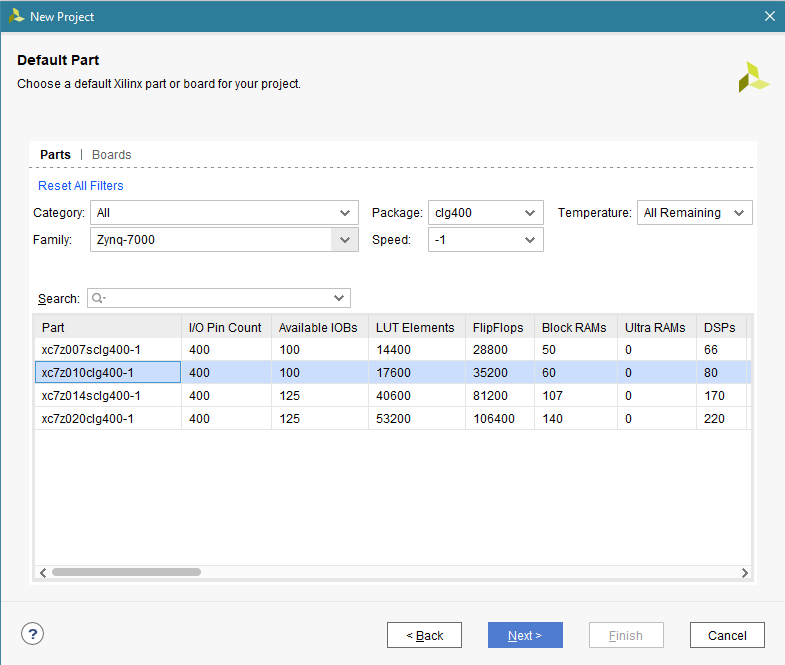
\includegraphics[width=.7\textwidth]{boards}
			\caption{Default Part Selection}
			\label{boards}
		\end{figure}
		
		
		
	\end{enumerate}
	
	\item Create a Verilog source file which describes the binary counter.
	
	\begin{enumerate}
		\item Right-click on the Design Sources within the Hierarchy window under Sources and select `Add Sources...' as shown in Figure~\ref{source_mux}.
		
	\begin{figure}[!h]
		\centering
		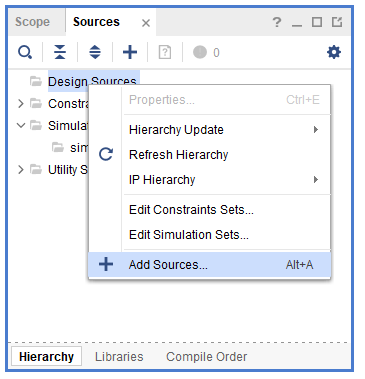
\includegraphics[width=.4\textwidth]{source_mux}
		\caption{Add Design Source}
		\label{source_mux}
	\end{figure}
		
		\item A window will appear. Select 'add or create design sources'. Click on the blue `+' button and select `Create file'. Type the name as `counter.v' and click 'OK'. Then click 'Finish'. A 'Define Module' window will come up. Click 'Ok' and 'Yes'. We are going to manually define our module with Verilog code. 
		\item In the hierarchy window under Design Sources you should see your counter module. Double click this module name to open the file in  the Vivado text editor window. 
		\item Type the following Verilog code into the Vivado text editor. \\
		
		\begin{minipage}{\linewidth}
			\lstinputlisting{counter.v}
		\end{minipage}
		
		
		\textbf{Note:} Do \textbf{NOT} copy and paste text from the PDF into the editor window. Symbols within the code do not always copy properly and will cause syntax errors when you attempt to build the project.
		
		
	\end{enumerate}
	
	\item Create a test bench to test the counter module.
	\vspace{-1em}
	\begin{enumerate}
		\item As we did with counter.v, add a new design source called "counter\_tb.v". Open the file and type the following lines into it. 
		
		\begin{minipage}{\linewidth}
			\lstinputlisting{counter_tb.v}
		\end{minipage}  
		
		\item  Ensure the hierarchy appears as seen in Figure~\ref{heirarchy}.
		
		\begin{figure}[!h]
			\centering
			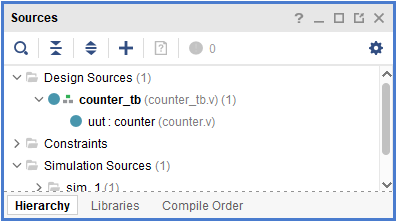
\includegraphics[width=.5\textwidth]{heirarchy}
			\caption{Source Heirarchy}
			\label{heirarchy}
		\end{figure}
		
		
		\item The test bench instantiates the unit under test (UUT), in this case our counter module, and applies inputs to it and monitors its outputs. This particular test bench cycles the clk input three times, and each time checks to see if the count output has incremented. If the counter ever outputs an incorrect count value, the test bench will print an error statement. If the counter outputs a correct value, the test bench will print a statement indicating that particular test has passed.
	\end{enumerate}

\begin{figure}[!ht]
	\centering
	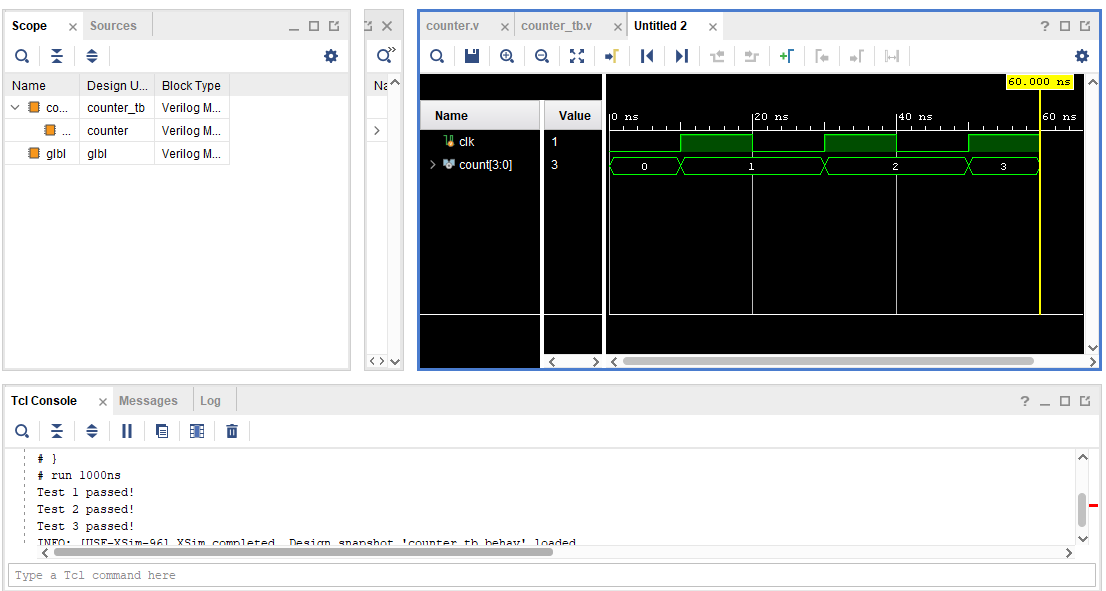
\includegraphics[width=.9\textwidth]{wave}
	\caption{Simulation Waveform for Counter Module}
	\label{wave}
\end{figure}
	
	\item Simulate the counter.
	\begin{enumerate}
		\item To simulate a file using a test bench, right click on the test bench file and select `Set as Top'. Here right click on `two\_one\_mux\_tb.v' and make it top.
		\item Click `Run Simulation' from within the Flow Navigator panel. Select `Run Behavioral Simulation'. 
		\item If there are any errors or warnings, they will show up in the Console panel. Correct any errors and warnings at this time. You may re-run the simulation process once you have fixed your source code.
		\item The waveform panel shown in Figure~\ref{wave} will open once your design successfully compiles. Take note of the waveform panel in the top-right corner and the console panel at the bottom. For this simulation, the waveform will be very simple. You may have to zoom in to see the values. Check the Tcl console output at the bottom of the screen to ensure that your design passes all of these tests. 
	
		
		
	\end{enumerate}
	
\end{enumerate}

\section{Connecting Ports and Programming the Zybo Z7-10 }

	\noindent
	In the previous section, we created a counter module in Verilog and simulated its operation. In this section, we will upgrade that module, then program it onto the FPGA on the Zybo Z7-10 board. This will create our counter in real hardware on the board, so that we are no longer simulating its behavior, but observing the real thing! \\
	
	
	\noindent
	Before we start, rewrite your module to contain the following text.
	
	\begin{minipage}{\linewidth}
		\lstinputlisting{counter2.v}
	\end{minipage}  
	
		\noindent
		In the context of the Zybo Z7-10 board, a "port" is a connection that can attach to an input or output of a Verilog module. Most ports can be seen on the front of your Zybo Z7-10 board. Some of the ports available to us are the push buttons and switches (module inputs) and LEDs (module outputs). Other important ports are the PMOD ports, which are the black rectangular prisms located along the edge of the board. PMOD ports allow us to attach physical wires to our module, which can be connected to either module inputs or outputs.\\
		
		\noindent
		Every port has a PIN to distinguish it. Using a Xilinx Design Constraints (XDC) file, we will indicate which ports are connected to the inputs and outputs of our module. We will now create an XDC file that connects the LEDs and one push button to our module.
		
		
		\begin{enumerate}
			
			\item Create an XDC file.
			\begin{enumerate}
				
				\item Right-click on the Design Sources within the Hierarchy window under Sources and select `Add Sources...' as we did before.
				\item This time, click "Add or create constraints".
				\item Click the blue '+' sign, click "Create constraints" and add a contraints file called "counter.xdc". Type the following lines into it.
				
				\begin{minipage}{\linewidth}
					\lstinputlisting{counter.xdc}
				\end{minipage} 
		
			\end{enumerate}
		
			\item Generate bitstream and program the Zybo Z7-10 FPGA.
			
			\begin{enumerate}
				
				\item A bitstream is a long string of bits which essentially tells the Field-Programmable Gate Array (FPGA) which connections in its large array of gates it should make to realize the hardware module we describe in Verilog. To generate the bitstream, under the Flow Navigator click "Generate Bitstream". This may take several minutes. 
				
				\item Before we program the Zybo Z7-10 board, we need to open a target. Connect your Zybo Z7-10 board to your computer's USB port and turn it on. Under the Flow Navigator, click "Open Target" and then "Open new target...". Click "Next" until you see a window that looks like Figure~\ref{target}. Click "xc7z010\_1" and click "Next" and then "Finish" to open our Zybo Z7-10 board as the hardware target.
				
				\begin{figure}[!h]
					\centering
					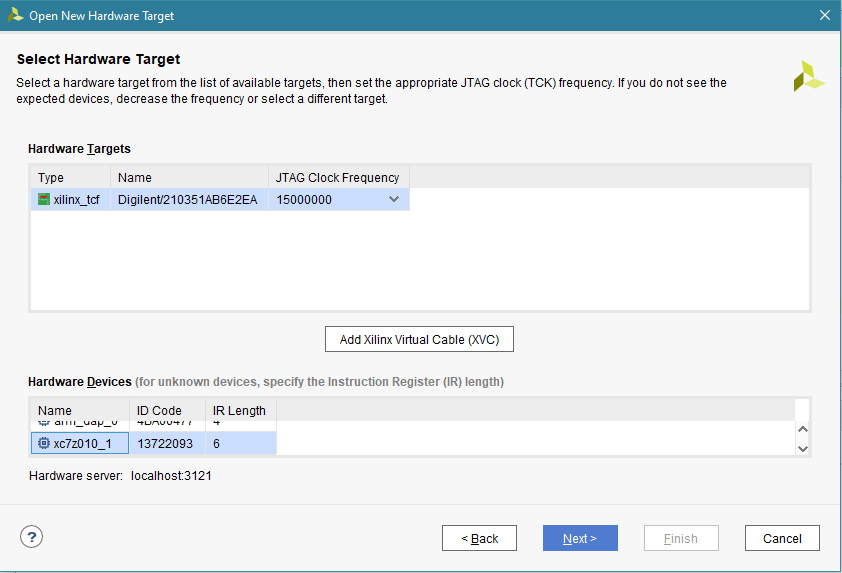
\includegraphics[width=.9\textwidth]{target}
					\caption{Open a Hardware Target}
					\label{target}
				\end{figure}
				
			\item We are now ready to program the Zybo Z7-10 board. Under the Flow Navigator click "Program Device". When Vivado is done with the programming, hold down BTN0 (the rightmost push button, port K18) and you should see the LEDs counting up. When you let go of the button, the LEDs should all turn off.
				
			\end{enumerate}
		
		\end{enumerate}


\section{Block Design Creation and Using the SDK}

	\textbf{Note:} The instructions in this section are very similar to the ECEN 449/749 lab 2 instructions.\\

	\noindent
	In the previous section, we synthesized a Verilog module onto the Zybo Z7-10 FPGA. Our module controlled the LEDs based on a binary counter created in hardware. In this section, we will accomplish similar functionality, but we will control the LEDs using software running on the Zybo Z7-10 board's processor.\\
	
	\begin{enumerate}
		
		\item In the following steps we will launch Vivado 2018 (on your home computer) and  create a block design. \\
		\begin{enumerate}
			\item Before beginning, create a directory for this project. Avoid spaces and special characters in the directory name as they have the potential for causing problems during the system build process.
			
			
			\item Launch Vivado, select `Create New Project' and follow the same procedure as shown in the "Simple Verilog Source Code" section of this manual to create a new RTL project, except do not add a source file to the project. In this lab you will use Xilinx Microblaze Processor.
			
			\item On the left side, in the Flow Navigator under the IP Integrator section, click on 'Create Block Design'. A window opens where you can specify the name of your design. Leave the 'Directory' and the 'Specify source set' as they are. Click on the `OK' button. (Figure \ref{createbd})   
			\begin{figure}[h]
				\begin{center}
					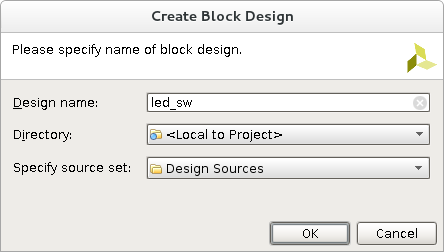
\includegraphics[width=0.6\textwidth]{lab24}
					\caption{Create Block Design}
					\label{createbd}
				\end{center}
			\end{figure}
			\item The Block Design Diagram opened (tab called Diagram) is empty. Right click within the diagram tab and select `Add IP'. Search `MicroBlaze' and double click on `MicroBlaze' to add it to our design. Right click and select 'Run Block Automation'. Select the following configuration for the MicroBlaze processor and click `OK'.
			(Figure \ref{microbla})   
			\begin{figure}[h]
				\begin{center}
					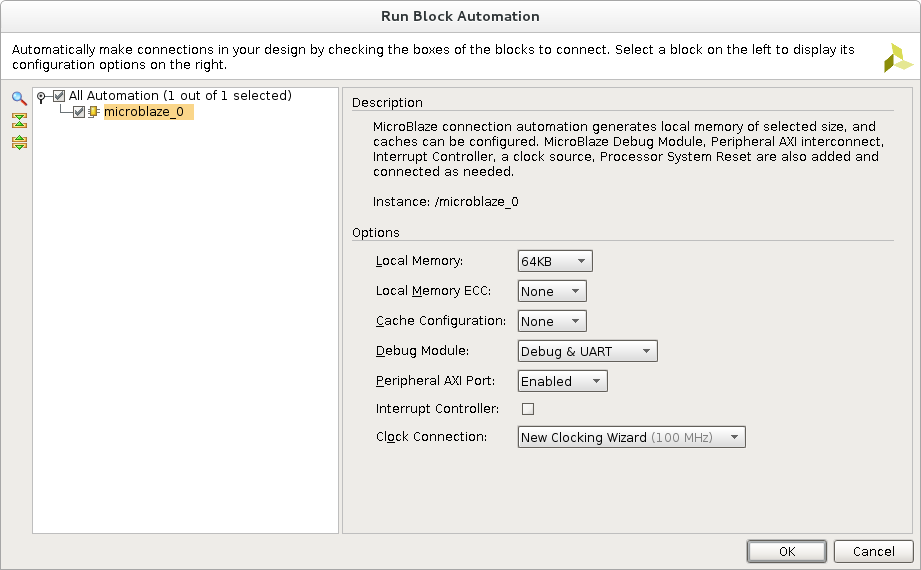
\includegraphics[width=0.8\textwidth]{lab2blockauto}
					\caption{Run Block Automation}
					\label{microbla}
				\end{center}
			\end{figure}
			
			
			Local Memory: 64KB\\
			Local Memory ECC: None\\
			Cache Configuration : None\\
			Debug Module: Debug \& UART\\
			Peripheral AXI Port: Enabled\\
			Interrupt Controller: Unchecked.\\ 
			Clock Connection: New Clocking Wizard (100 MHz)\\
			
			\item  Once the Diagram is generated, double-click on the `Clocking Wizard' block named `clk\_wiz\_1'. This launches the `Re-customize IP' window. Select `Clocking Options' and change the source of the `Primary Input Clock' from `Differential clock capable pin' to 'Single ended clock capable pin'. Click `OK'.  
			\item Right click and select `Run Connection Automation' in the diagram. In the `Run Connection Automation window' check `All Automation' and click `OK'. 
			\item The processor is set up, now we need to add a General Purpose IO (GPIO) block to interact with LEDS on the Zybo Z7-10 board. Right click and select `ADD IP'. Search for `GPIO' and select `AXI GPIO' to add it to the design. Double click on the GPIO block named `axi\_gpio\_0'. Set the following configuration for the GPIO and click `OK'
			(Figure \ref{gpio}).   
			\begin{figure}[h]
				\begin{center}
					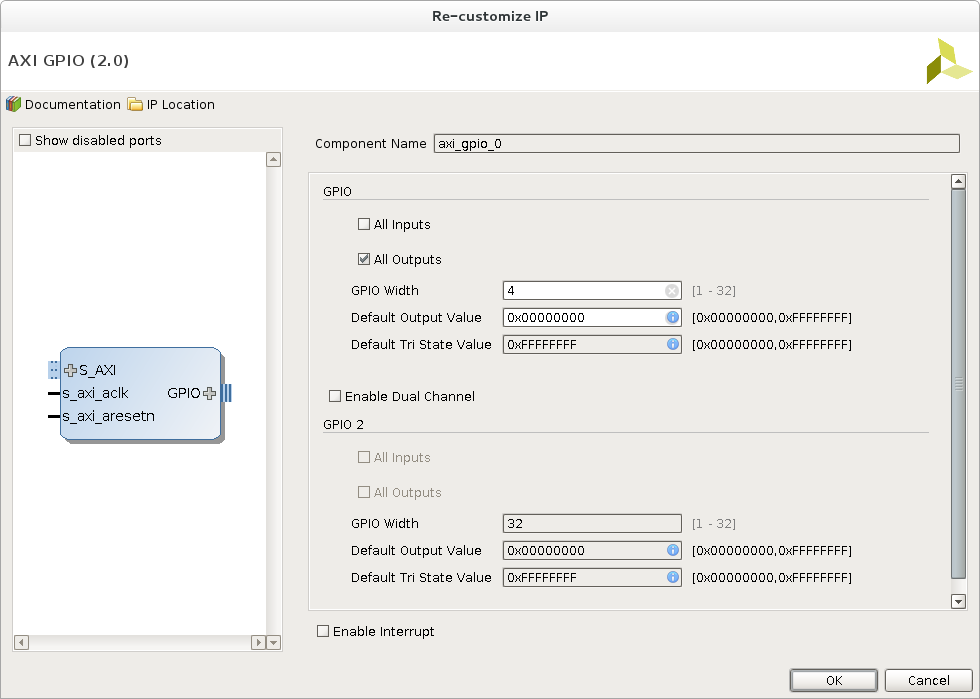
\includegraphics[width=0.8\textwidth]{lab2GPIOconf}
					\caption{Customize GPIO}
					\label{gpio}
				\end{center}
			\end{figure} 
			
			All Inputs: (not checked)
			
			All Outputs (checked)
			
			GPIO Width: 4
			
			Leave the remaining values unchanged.
			\item Right click and select `Run Connection Automation', check `All Automation', and click `OK'. Now  design is connected. To make it look neat, right click and select `Regenerate Layout'. 
			\item You are using the GPIO block to configure LEDs, so let's rename the `AXI GPIO' block. Select the `AXI GPIO' block and rename the block to `led' in the 'Block Properties' panel and press `Enter'. Repeat the same procedure for the port connected to the `AXI GPIO' block and rename it to `led'. The layout should look like Figure \ref{lay}   
			\begin{figure}[h]
				\begin{center}
					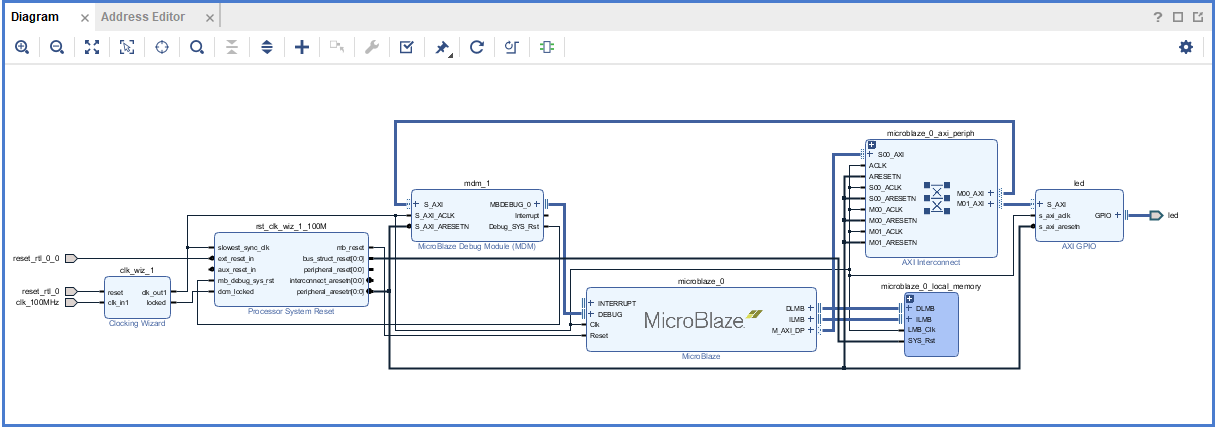
\includegraphics[width=1.0\textwidth]{diagram}
					\caption{Layout}
					\label{lay}
				\end{center}
			\end{figure} 
			\item  Double click the `reset\_rtl\_0' port in the diagram. You can see that it is `ACTIVE LOW'. Double Click on the `reset\_rtl' port and observe that it is `ACTIVE HIGH'.
			\item These are the reset ports for Microblaze. On Zybo Z7-10 board we have dedicated reset pins for reset. Refer to manual and see the functionality of  BTN6 and BTN7.
			\item These two reset ports can be configured to a push button on the board. For the purpose of this lab,  connect the ports to constant values and use the dedicated pins on board for reset.
			\item Select `Constant' IP from the IP repository (Right click and ADD IP) and add two instances to the diagram. Double click on one of the constant IP blocks and set `Constant Width' to 1 and `Constant Value' to 1. Rename this block to `VDD'. Now, right click on the `reset\_rtl\_0'  port and  select `Delete' to delete it. Connect the constant block to `ext\_rst\_in' of the `Processor System Reset' because it is  `ACTIVE LOW'. Connect the constant block by clicking on the output of the constant block and dragging it to the `ext\_rst\_in' pin. 
			\item Repeat the same procedure for the other constant block but set `constant value' to 0 and rename it as `GND'. Delete the  `reset\_rtl' port and connect it to the `reset' port of the `Clocking Wizard'.
			
			
			\item  Right click on the diagram and select `Regenerate Layout'. The final layout should look like Figure \ref{lay1}.  
			
			
		\end{enumerate}  
		\item In the following steps we map the IO ports to the LEDs and buttons.  
		\begin{enumerate} 
			
			\item In the design tab, expand `External Interfaces' and `Ports' and examine the ports listed. When `led' is expanded it shows the `led\_tri\_o'and `clock\_100MHz' ports listed. We need to connect these ports to the Zybo Z7-10 board.
			
			\item  In the sources panel, right click on the constraints  and select `Add sources'. Next, in the add sources window, select  `Add or create constraints' and click `Next'. Click on the green `+' button and select `create file'. The `Create Constraints File' window will open, give a file name (eg. led), and click `OK'. Select `Finish' to create a constraint file.
			\item In the sources panel, expand `Constraints' and double click on the created XDC file to open it.
			\item Add the following code to attach the above ports to the pins on Zybo Z7-10 board. 
			\begin{lstlisting}
			
#clock_100MHz
set_property PACKAGE_PIN K17 [get_ports clock_100MHz]
set_property IOSTANDARD LVCMOS33 [get_ports clock_100MHz]
create_clock -add -name sys_clk_pin -period 10.00 -waveform {0 5} [get_ports clock_100MHz]


#led_tri_o
set_property PACKAGE_PIN M14 [get_ports {led_tri_o[0]}]
set_property IOSTANDARD LVCMOS33 [get_ports {led_tri_o[0]}]


set_property PACKAGE_PIN M15 [get_ports {led_tri_o[1]}]
set_property IOSTANDARD LVCMOS33 [get_ports {led_tri_o[1]}]


set_property PACKAGE_PIN G14 [get_ports {led_tri_o[2]}]
set_property IOSTANDARD LVCMOS33 [get_ports {led_tri_o[2]}]


set_property PACKAGE_PIN D18 [get_ports {led_tri_o[3]}]
set_property IOSTANDARD LVCMOS33 [get_ports {led_tri_o[3]}]
			\end{lstlisting}
			
			\begin{figure}[h]
				\begin{center}
					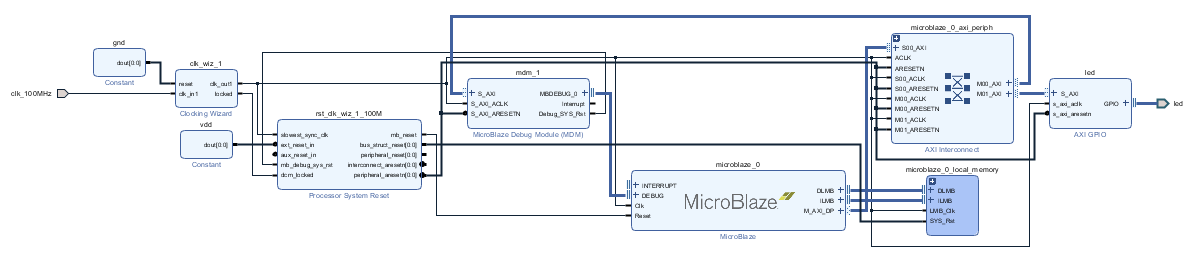
\includegraphics[width=1.0\textwidth]{lab2final}
					\caption{Final Layout}
					\label{lay1}
				\end{center}
			\end{figure}
			
			
		\end{enumerate}
		\item In the following steps we will Generate Bitstream and launch the SDK.
		\begin{enumerate}
			
			
			\item Right click in the diagram and select 'Validate Design' to check for any errors in the design. If everything is correct, you have successfully built the hardware platform. 
			\item Right click on your project in the sources panel and select `Create HDL wrapper'. Select `Let Vivado manage wrapper and auto update'  and click `OK' to create the top level module for the design. Finally,  click `Generate Bitstream' to create the program file. Once this is done, we will be able to export our hardware design and switch over to the SDK to program the FPGA and run the program to manage LEDs.
			\item If any errors are found please rectify them. Once successfully completed, select File $\rightarrow$ `Export'  $\rightarrow$ `Export Hardware'. Check `Include bitstream' to export the hardware platform.
			\item Now, launch the Software Development Kit(SDK) using `File' $\rightarrow$ `Launch SDK'. Select `local to project' as the location.
			
		\end{enumerate}
		
		\item In the following steps we will use the SDK to create the software application.
		\begin{enumerate}
			
			\item Once the SDK is open, wait for it to import hardware specification. Then, select `File' $\rightarrow$ `New' $\rightarrow$ `Application Project'. Give a project name (eg.counter\_sw). Click `Next' and select the `Empty Application' and click `Finish'.
			\item You will now have three files in the 'Project Explorer' panel (counter\_sw, counter\_sw\_bsp and led\_wrapper\_hw\_platform\_0). 
			\item Using your favorite editor, create a file called `led\_cntrl.c'. Type the  C code shown below in your file and save it in your project directory.
			\begin{lstlisting}
#include <xparameters.h>
#include <xgpio.h>
#include <xstatus.h>
#include <xil_printf.h>
/* Definitions */
#define GPIO_DEVICE_ID  XPAR_LED_DEVICE_ID	/* GPIO device that LEDs */
                                        	/* are connected to  */
#define WAIT_VAL 10000000				

int  delay (void) ;

int main()
{
	int count;
	int count_masked;
	XGpio leds;
	int status;
	
	status=XGpio_Initialize(&leds,GPIO_DEVICE_ID);
	XGpio_SetDataDirection(&leds,1,0x00);
	if (status != XST_SUCCESS) {
		xil_printf("Initialization failed");
	}
	count=0;
	while(1)
	{
		count_masked=count & 0xF ;
		XGpio_DiscreteWrite(&leds,1,count_masked);
		xil_printf("Value of LEDs = 0x%x\n\r", count_masked);
		delay();
		count++;
	}
	return(0);
}

int delay(void)
{
	volatile int delay_count=0;
	while(delay_count < WAIT_VAL)
	delay_count++;
	return (0);
}
			
			
			\end{lstlisting}
			\item Look through the code you just wrote and try to understand what exactly is going on. Notice we include the `xparameters.h', `xstatus.h', and `xgpio.h' header files.  Open up these files from  the `Outline' panel to the right of the window and understand what they provide. Specifically, look at the XGpio functions we call and understand how they work.
			
			\item In the project explorer, expand `counter\_sw', right click on `src' and select `import'. In the import window expand `General', select `File System', and click `Next'. Click `Browse' and select the folder where you saved the led\_cntrl.c file and click `OK'. Select the led\_cntrl.c file from the import window and click `Finish'.
			\item Now we have the software application ready. Connect the FPGA and switch it ON. In the SDK, click `Xilinx' and select `Program FPGA'. Next, the `Program FPGA' window will appear and select 'Program' to program the the bitstream file generated in Vivado on to the FPGA. A warning will appear indicating that there is no PS in the design. PS is short for processing system which represents the ARM Cortex Processor in the Zybo Z7-10 board. In this lab, the Microblaze processor is used which is implemented completely on the FPGA, and hence it is called a soft processor. Click `OK' on the message to program the FPGA.
			
			\item The next step is to run the C application on the system. Under `counter\_sw' in the Project Explorer expand `binaries'. Right click on `counter\_sw.elf', select `Run As' and click on `Launch on Hardware(System Debugger)'. This command creates a configuration file which we can use to run our application. Vivado will launch the application on the Zybo Z7-10 board.
			
			\item If everything is correct, you should now be able to see the LEDs glowing in the order from 0 to 15 and the output from the printf statements  on the console in the SDK.
			NOTE: For the purpose of debugging stop the program by entering `stop' on the XSCT console and re-run the program. The XSCT console can be found under `Xilinx'.
		\end{enumerate}   
		
	\end{enumerate}
	











\section{Custom IP Creation}

\noindent
\textbf{Note:} The instructions in this section are very similar to the ECEN 449/749 lab 3 instructions.\\

\noindent
In this section, we will create our own custom IP (intellectual property) block. This block will be connected to 3 registers. It will use two of these registers as inputs (slv\_reg0 and slv\_reg1), and one as output (slv\_reg2). The function of this block will be simple: to multiply the value stored in slv\_reg0 with the value stored in slv\_reg1 and store that value in slv\_reg2.\\

\noindent
The 3 registers will be software-accessble, which means that software running on the Zybo Z7-10 board's processing system will be able to write values to these registers. We will create a simple program that writes values to the multiply IP's input registers and reads the multiplied result from its output register.\\

\noindent
Create Zynq Base System (in Vivado 2018 on your local pc)
\begin{enumerate}
	
	\item To begin, open Vivado and create a new project as shown in  in the "Simple Verilog Source Code" section of this document.
	
	\item Click on `Create Block Design' and name the design `multiply'. In the diagram, add `ZYNQ7 Processing System' IP as in Figure \ref{zynq}.
	
	\begin{figure}[!h]
		\begin{center}
			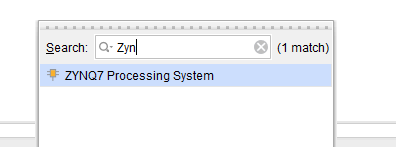
\includegraphics[width=0.7\textwidth]{zynq}
			\caption{Zynq Processing System}
			\label{zynq}
		\end{center}
	\end{figure}

	Double click on the PS IP to open `Re-customize IP' window. 
	Download the `ZYBO$\_$Z7$\_$B2$\_$.tcl' file 
	from /mnt/lab\_files/ECEN449 and save this TCL 
	file somewhere on your local computer. 
	In the `Re-customize IP' window, click on `Presets $\rightarrow$ Apply Configuration', 
	and import the TCL file you just downloaded. 
	Then click on `Peripheral I/O Pins' tap, and uncheck all the peripheral I/O pins.
	
	\item In the `Re-customize IP' window, click on `Peripheral I/O Pins'. To build the hardware depicted in Figure\ref{zynq}. Enable `UART 1' by clicking on the check box. Double check and make sure that only the `UART 1' is selected.
	
	\item Click on `Zynq Block Design' tab and observe the diagram. Note that the `Application processing Unit' which represent the ARM processors on the Zybo Z7-10 board is connected to `UART 1' through a `Central Interconnect' block. Click `OK'
	
	\item PS is ready and the next part is to create the `multiply' IP. Click on `Tools' and select `Create and Package IP'. This will open `Create and Package New IP' window  and click on  `Next'. Now select `Create a new AXI4 peripheral' and click on 'Next'.
	
	\item A window will appear prompting you to assign a name and 
	version number to your peripheral (Figure\ref{ip}). 
	Name the peripheral `multiply' and leave 
	the version number as default (i.e 1.0). Then, click on `Next'.
	
	\begin{figure}[!h]
		\begin{center}
			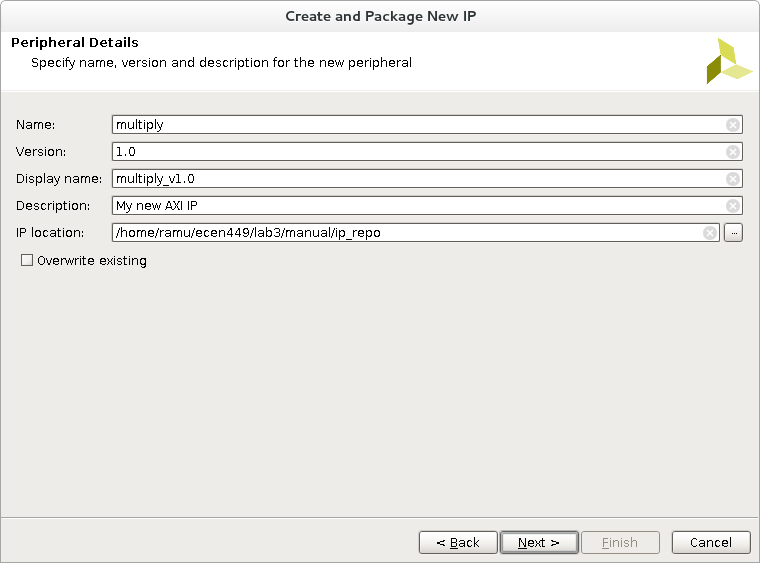
\includegraphics[width=0.8\textwidth]{ip}
			\caption{Create New IP}
			\label{ip}
		\end{center}
	\end{figure}
	
	\item The next window will ask us to select `Interface'. Leave the default values\\
	Interface type : Lite\\ Interface mode: slave \\ Data Width: 32 \\ Number of Registers: 4\\  We will need only three registers for the `multiply' IP however the minimum number of registers allowed is 4 (see Figure \ref{ip_interface}, Click on `Next'. You will see a summary of the IP we have created. We still need to add the functionality of the multiplier to this IP. Check `Edit IP' and click `Finish'. Another Vivado window will open which will allow you to modify the peripheral that we created. 
	\begin{figure}[h]
		\begin{center}
			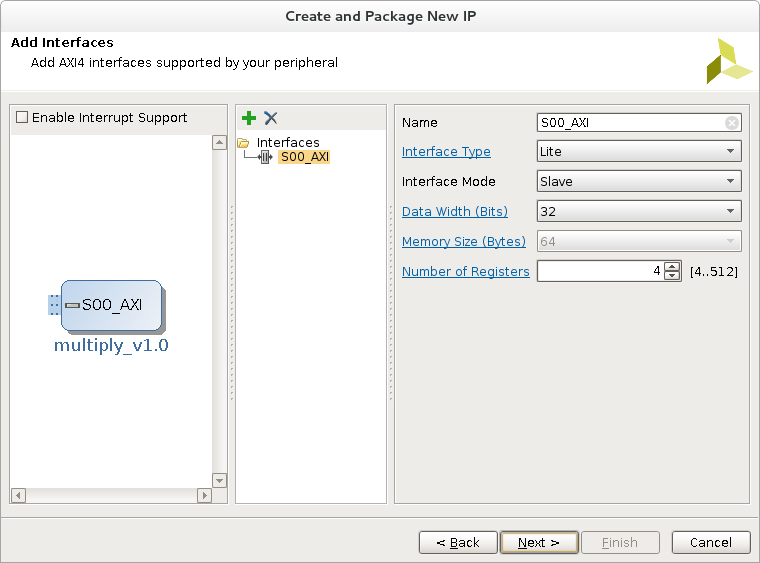
\includegraphics[width=0.8\textwidth]{ip_interface}
			\caption{ IP Interface Options}
			\label{ip_interface}
		\end{center}
	\end{figure}
	\item At this point, the peripheral that has been generated by Vivado is an AXI lite slave that contains 4 x 32 bit read/write registers. We want to add our multiplier code to the IP and modify it so that two of the registers connect to the multiplier inputs and another register connects to the multiplier output.
\end{enumerate}
Edit `multiply' IP and Import it to PS
\begin{enumerate}
	
	\item Open the new Vivado window that contains the peripheral we created (not the base project). Review the information under the various tabs in the Package IP tab.
	\item In the sources window, expand `multiply\_v1\_0' and double click on the `multiply\_v1\_0\_S00\_AXI.v' file to open it.
	
	\item Examine the verilog code in file and try to understand each function, especially how the `read' and `write' functions are implemented. Comment out any code that writes to `slv\_reg2'(i.e.` slv\_reg2 $<=$'). This will deactivate the write capabilities to the third software register which is our multiplier output. Remember that we cannot have two drivers for a particular register unless we add multiplexing logic.
	
	\item While the `multiply\_v1\_0\_S00\_AXI.v' file is still open, locate the \\
	`// Add user logic here' line and insert the
	following code:
	\begin{lstlisting}
reg [0 : C_S_AXI_DATA_WIDTH-1] tmp_reg ;
always @( posedge S_AXI_ACLK ) begin
	if( S_AXI_ARESETN == 1'b0 ) begin
		slv_reg2 <=0;
		tmp_reg <=0;
	end
	else begin
		tmp_reg <= slv_reg0 * slv_reg1;
		slv_reg2 <= tmp_reg ;
	end
end
	\end{lstlisting}
	
	Examine the above code, comment it appropriately, and save it.
	\item In Package IP tab, click on `Review and Package' and select `Re-package'. Now Vivado will repackage the IP with added functionality. When Vivado finishes packaging the IP, close the project.
	
	\item At this point in the lab, we have used Vivado to generate template hardware peripheral files for our multiplication peripheral based on our specifications. We have also added user logic in Verilog to our template for the multiplication functionality of our peripheral. We are now ready to import our peripheral into Vivado and add it to our PS system.
	
	\item Now, select the Vivado window which has the PS system. Open the diagram tab and add `multiply' IP to the PS system. Select `Run Connection Automation' and in the prompted window select `All Automation' and click `OK'. Once automation is completed, a layout is generated. Right click on the diagram and select `Regenerate Layout' to redraw the layout design. The layout is shown in Figure\ref{lay}. A `Processor System Reset' block is also created which synchronizes the peripheral and interconnect reset to clock.
	
	\begin{figure}[!h]
		\begin{center}
			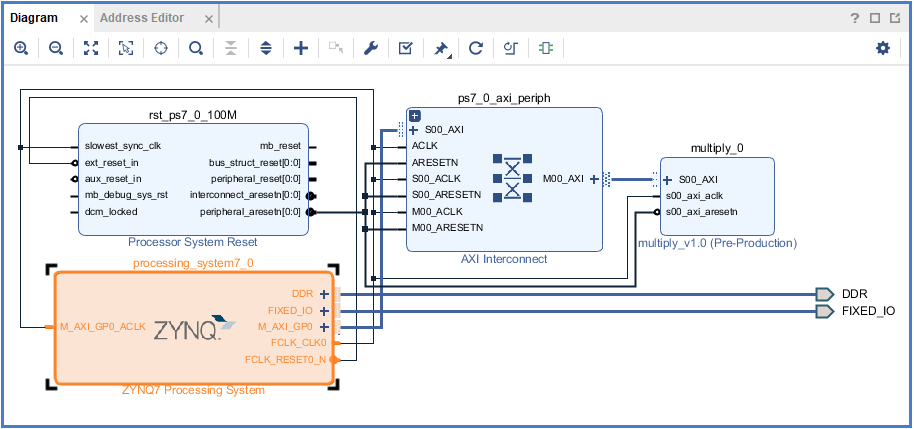
\includegraphics[width=1.0\textwidth]{layf}
			\caption{ Layout of the Design}
			\label{lay}
		\end{center}
		
	\end{figure}
	
	\item In the source tab, right click on your block 
	design and select `Create HDL wrapper'. 
	In the `Create HDL wrapper' window 
	select `Let Vivado manage wrapper and auto update'. 
	This will create the top module for the blocks 
	in the block diagram. Click `OK'
	Ignore any critical messages during the process.
	
	\item Now we have the PS system and multiply IP ready. 
	It is time to generate the bitstream. 
	In the Flow Navigator, select `Generate Bit Stream'. 
	
	\item Once the bit generation is complete, 
	it is time to write an application and test the multiply IP.
	
	\item Export the design including bit stream as shown in the "Block Design Creation and Using the SDK" section of this document.
	
	
\end{enumerate}
Launch SDK (File $\rightarrow$ Launch SDK) and write multiplication test application.
\begin{enumerate}
	\item Currently, our hardware should be ready to go. Next step is to create an application to test our `multiply' IP peripheral. Open the SDK and click on `File' and select `New' $\rightarrow$ `Application Project'. In the new project window, give a name(eg. multiply\_test) to the project and leave the default values for the remaining fields. Click `Next' and select `Hello World!' and `Finish'. This step will generate the necessary templates files for our PS on the Zybo Z7-10 board. 
	\item In the project explorer, expand 'multiply\_test'. Under the src folder, open `helloworld.c' file and examine the code generated. 
	
	\item Edit the `helloworld.c' source file to look like the code below.
	
	\begin{lstlisting}
	
	
#include <stdio.h>
#include "platform.h"
#include <xparameters.h>
#include "multiply.h"
#include "xil_printf.h"
#include "xil_io.h"

#define BASEADDR XPAR_MULTIPLY_0_S00_AXI_BASEADDR
#define REG0_OFFSET MULTIPLY_S00_AXI_SLV_REG0_OFFSET
#define REG1_OFFSET MULTIPLY_S00_AXI_SLV_REG1_OFFSET
#define REG2_OFFSET MULTIPLY_S00_AXI_SLV_REG2_OFFSET

int main()
{
	init_platform();
	
	int i;
	for(i = 1; i <=16; i++)
	{
		// This will write i to slv_reg0
		MULTIPLY_mWriteReg(BASEADDR, REG0_OFFSET, i);
		
		// This will write i to slv_reg1
		MULTIPLY_mWriteReg(BASEADDR, REG1_OFFSET, i);
		
		// This will read the value from slv_reg2, which should be i*i
		xil_printf("%d, ", MULTIPLY_mReadReg(BASEADDR, REG2_OFFSET));
	}
	xil_printf("\n");
	
	cleanup_platform();
	return 0;
}
	
	\end{lstlisting}
	
	\item Note that you can open a file by Ctrl-clicking on the include statement for that file. You can also expand the "Includes" dropdown under your project in the "Project Explorer" panel on the left of the SDK screen. Open "multiply.h" and examine its contents. Specifically, see what values it has set for the register offsets, like MULTIPLY\_S00\_AXI\_SLV\_REG0\_OFFSET (henceforth referred to as 'REG0\_OFFSET'). Open "xparameters.h" and find the definition of XPAR\_MULTIPLY\_0\_S00\_AXI\_BASEADDR (henceforth referred to as 'BASEADDR').
	
	\item The BASEADDR defined in xparameters.h and offsets defined in multiply.h are used when we write (with MULTIPLY\_mWriteReg()) or read (with MULTIPLY\_mReadReg()) to our multiply registers (slv\_reg0, slv\_reg1, and slv\_reg2). For instance, when we call MULTIPLY\_mWriteReg with BASEADDR and REG0\_OFFSET, the function can compute the exact memory location of slv\_reg0, which is BASEADDR $+$ REG0\_OFFSET.
	
	\item Once you have written the source file,  save it under src folder. Make sure your Zybo Z7-10 board is connected to your computer and powered on. Click on `Xilinx Tools' and select `Program FPGA' to program the bitstream file to the Zybo Z7-10 board. Click `Program'. 
	
	\item In order to see our program output, we will need to connect a terminal to the PS UART. Open a MobaXterm and create a serial connection to port COM4. If you are unsure how to do this, refer to the "MobaXterm and SSH How-To Document".
	
	\item Under `multiply\_test' expand `binaries'. Right click on `multiply\_test.elf', select `Run As' and click on `Launch on Hardware(System Debugger)'. This command creates a configuration file which we can use to run our application. Vivado will launch the application on the Zybo Z7-10 board.
	
	
	If everything is correct, you will see text being printed to the SDK Terminal, which is a list of squares from $1^2$ to $16^2$, as shown in Figure~\ref{mult_output}. \\
	
		\begin{figure}[!h]
		\begin{center}
			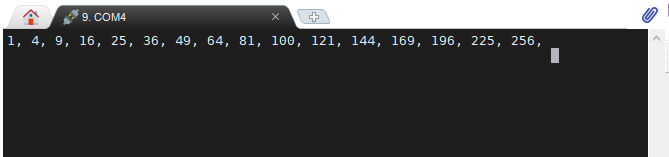
\includegraphics[width=0.7\textwidth]{mult_output}
			\caption{Output of the Multiply Test Application}
			\label{mult_output}
		\end{center}
		
	\end{figure}

\end{enumerate}	


\end{document}

